% Copyright (c) 2015-2021 Robert Ryszard Paciorek <rrp@opcode.eu.org>
% 
% MIT License
% 
% Permission is hereby granted, free of charge, to any person obtaining a copy
% of this software and associated documentation files (the "Software"), to deal
% in the Software without restriction, including without limitation the rights
% to use, copy, modify, merge, publish, distribute, sublicense, and/or sell
% copies of the Software, and to permit persons to whom the Software is
% furnished to do so, subject to the following conditions:
% 
% The above copyright notice and this permission notice shall be included in all
% copies or substantial portions of the Software.
% 
% THE SOFTWARE IS PROVIDED "AS IS", WITHOUT WARRANTY OF ANY KIND, EXPRESS OR
% IMPLIED, INCLUDING BUT NOT LIMITED TO THE WARRANTIES OF MERCHANTABILITY,
% FITNESS FOR A PARTICULAR PURPOSE AND NONINFRINGEMENT. IN NO EVENT SHALL THE
% AUTHORS OR COPYRIGHT HOLDERS BE LIABLE FOR ANY CLAIM, DAMAGES OR OTHER
% LIABILITY, WHETHER IN AN ACTION OF CONTRACT, TORT OR OTHERWISE, ARISING FROM,
% OUT OF OR IN CONNECTION WITH THE SOFTWARE OR THE USE OR OTHER DEALINGS IN THE
% SOFTWARE.

\section{Obwody prądu zmiennego}

W elektronice (zwłaszcza analogowej) spotyka się z obwodami prądu zmiennego, jednak są to na ogół sygnały zmienne i wartość płynącego prądu (a co za tym idzie także mocy) nie jest znaczna. Inaczej sytuacja wygląda w instalacjach elektrycznych gdzie typowo mamy prąd przemienny (50Hz lub 60Hz, zależnie od rejonu świata) oraz spore wartości napięcia, prądy i moce. W związku z tym spojrzenie elektryka jest trochę inne niż elektronika – nie ma np. większego znaczenia pasmo częstotliwości danego układu, a istotne jest przesuniecie fazowe pomiędzy prądem a napięciem oraz związane z tym zagadnienia mocy biernej i pozornej.

\subsection{Wartość szytowa, międzyszczytowa, skuteczna i amplituda}

\begin{center} \begin{adjustbox}{scale=1.0} \begin{tikzpicture}
	\begin{axis}[
		axis lines=middle,
		unit vector ratio*=1 1,
		scale=2.3,
		ymin=-1.9, ymax=1.9, xmin=-3.5, xmax=7,
		domain=-3.5:7,
		samples=100,
		ymajorticks=false,
		xmajorticks=false,
		disabledatascaling
	]
	\addplot [mark=none] {sin(deg(x))};
	
	\draw[dashed] (-pi, 1)  -- (2*pi, 1);
	\draw[dashed] (-pi, 0.7071)  -- (2*pi, 0.7071);
	\draw[dashed] (-pi, -1) -- (2*pi, -1);
	
	\draw[<->, line width=0.35mm, green] (-0.5*pi, -1) -- (-0.5*pi, 1);
	\node[anchor = south, align = center, green] at (-0.5*pi, 1.0) {wartość międzyszczytowa\\\textit{peak to peak}};
	
	\draw[<->, line width=0.35mm, blue] (0.5*pi, 0) -- (0.5*pi, 1);
	\node[anchor = south, align = center, blue] at (0.5*pi, 1.0) {wartość szczytowa\\\textit{peak}};
	
	\draw[<->, line width=0.35mm, red] (1.5*pi, 0) -- (1.5*pi, 0.7071);
	\node[anchor = south, align = center, red] at (1.5*pi, 1.0) {wartość skuteczna\\\textit{RMS}};
	
	\draw[purple, dashed] (0, 0) -- (0, -1.6);
	\draw[purple, dashed] (2*pi, 0) -- (2*pi, -1.6);
	\draw[<->, purple]    (0, -1.3) -- node[below] {okres $T = 1/f$} (2*pi, -1.3);
\end{axis}
\end{tikzpicture} \end{adjustbox} \end{center} \vspace{-0.3cm}

\subsubsection{Wartość międzyszczytowa (peak to peak)}

Wartość międzyszczytowa jest to różnica pomiędzy wartością maksymalną a minimalną sygnału. Nie uwzględnia ona składowej stałej.

\subsubsection{Wartość szyszczytowa (peak)}

Maksymalna wartość sygnału względem poziomu odniesienia (np. zera lub poziomu składowej DC).
Zależnie od przyjętego poziomu odniesienia może uwzględniać, uwzględniać częściowo lub nie uwzględniać składowej stałej.

Dla symetrycznych przebiegów okresowych (takich jak sinusoidalny, prostokątny lub trójkątny) bez składowej stałej wartość szczytowa stanowi połowę wartości międzyszczytowej i jest równa \href{https://en.wikipedia.org/wiki/Amplitude}{\strong{amplitudzie}} sygnału. Jest to też maksymalna wartość napięcia uzyskanego w wyniku wyprostowania napięcia przemiennego\footnote{w rzeczywistości będzie pomniejszona o spadek napięcia na układzie prostującym}.

\subsubsection{Wartość skuteczna (RMS)}

\href{https://pl.wikipedia.org/wiki/Warto\%C5\%9B\%C4\%87_skuteczna}{Wartość skuteczna} $I_{sk}$ prądu przemiennego (opisanego funkcją $i(t)$) jest to wartość prądu stałego równoważnego mu pod względem wydzielenia takiej samej mocy w trakcie pełnego okresu.

\noindent
Moc prądu stałego wydzielana w czasie T: $$P = {I_{sk}}^2RT$$
Moc prądu przemiennego wydzielana w czasie pełnego okresu T: $$P = \int\limits^{T}_{0}{i^2(t)Rdt}$$
Z porównania otrzymujemy:

$$I_{sk} = \sqrt{\frac{1}{T}\int\limits^{T}_{0}{i^2(t)}dt}$$

\noindent
Analogicznie napięcie skuteczne:
$$U_{sk} = \sqrt{\frac{1}{T}\int\limits^{T}_{0}{u^2(t)}dt}$$

\noindent
Dla przebiegu sinusoidalnego:
	$$I_{sk} = \frac{I_{pp}}{2\sqrt{2}} = \frac{I_{0}}{\sqrt{2}} \qquad\qquad U_{sk} = \frac{U_{pp}}{2\sqrt{2}} = \frac{U_{0}}{\sqrt{2}}$$
gdzie:
\begin{itemize}
	\item $I_{pp}$ – wartość międzyszczytowa natężenia prądu
	\item $I_{0}$  – amplituda (wartość szytytowa) natężenia prądu
	\item $U_{pp}$ – wartość międzyszczytowa napięcia
	\item $U_{0}$  – amplituda (wartość szytytowa) napięcia
\end{itemize}

Ze względu na równoważność efektów z prądem stałym wartości skuteczne są powszechnie stosowane do opisywania prądów przemiennych.
Także mierniki elektryczne prądu przemiennego podają wartości skuteczne natężenia i napięcia\footnote{
	Mierniki nie \textit{true RMS} podają je z zależności $I_{sk} = \frac{I_{0}}{\sqrt{2}}$, $U_{sk} = \frac{U_{0}}{\sqrt{2}}$,
		która jest prawdziwa tylko dla przebiegu sinusoidalnego.
	Mierniki \textit{true RMS} dokonują obliczenia „rzeczywistej” wartości skutecznej wykonując odpowiednio wiele próbkowań sygnału.
}.


\subsection{Impedancja}

\href{https://pl.wikipedia.org/wiki/Impedancja}{Impedancja} jest uogólnieniem oporu dla obwodów prądu przemiennego zawierających kondensatory (pojemności) i cewki (indukcyjności). Jest to wartość zespolona dana zależnością:

$$Z = R + jX$$

\noindent
gdzie:
\begin{itemize}
	\item $R$ – \strong{rezystancja},
	\item $X$ – \strong{reaktancja}:
	\begin{itemize}
		\item dla cewki: $X = \omega L$
		\item dla kondensatora: $X = - \frac{1}{\omega C}$
		\item gdzie:
		\begin{itemize}
			\item $L$ – indukcyjność cewki
			\item $C$ – pojemność kondensatora
			\item $\omega = 2 \pi f$ – częstość kołowa
			\item $f$ to częstotliwość prądu (w Hz)
		\end{itemize}
	\end{itemize}
	\item j – jedność urojona, $j^2 = -1$
\end{itemize}

\vspace{5mm}\noindent
Należy zwrócić uwagę na przeciwny znak reaktancji dla pojemności i indukcyjności.
Jest to związane ze znoszeniem się reaktancji (a zatem też impedancji) połączonych ze sobą kondensatora i cewki.
W związku z tym impedancja może mieć charakter pojemnościowy (gdy $X<0$), indukcyjny (gdy $X>0$)\footnote{
	w odbu wypadkach z możliwą jakąś wartością rezystancji
} lub czysto rezystancyjny (gdy $X=0$, czyli $Z=R$).

\begin{center} \begin{adjustbox}{scale=1.0} \begin{tikzpicture}
	\tikzstyle{invisibleNode}=[inner sep=0, outer sep = 0pt, minimum size=0]
	\begin{axis}[
		axis lines=middle,
		xlabel=$Re$,
		xmin=-1.5, xmax=3.5,
		xtick={      -1,   1},
		xlabel style={above, xshift=-1ex},
		ylabel=$Im$,
		ymin=-3.0, ymax=3.0,
		yticklabels={$-j$, $j$},
		ytick={      -1,   1},
		disabledatascaling
	]
		\node[invisibleNode] at (2.5,1.8) (Z) {};
		
		\draw[->, >={Stealth[length=8pt,width=6pt]}] (0,0) -- node[above] {$Z$} (Z);
		
		\draw[blue, dashed] (Z) -- (Z |- 0,0);
		\node[blue, anchor = north] at (Z |- 0,0) {R};
		
		\draw[red, dashed] (Z) -- (Z -| 0,0);
		\node[red, anchor = east] at (Z -| 0,0) {X};
		
		\draw ([shift=(0:1.3)]0,0) arc (0:36:1.3);
		\node at (0.9, 0.27) {$\phi$};
		
		\node[align=center] at (1.75, -2) {\small $Z$ ma charkter\\indukcyjny};
	\end{axis}
\end{tikzpicture} \end{adjustbox} \hspace{0.5cm} \begin{adjustbox}{scale=1.0} \begin{tikzpicture}
	\tikzstyle{invisibleNode}=[inner sep=0, outer sep = 0pt, minimum size=0]
	\begin{axis}[
		axis lines=middle,
		xlabel=$Re$,
		xmin=-1.5, xmax=3.5,
		xtick={      -1,   1},
		xticklabel style={above, yshift=0.5ex},
		xlabel style={below, xshift=-1ex},
		ylabel=$Im$,
		ymin=-3.0, ymax=3.0,
		yticklabels={$-j$, $j$},
		ytick={      -1,   1},
		disabledatascaling
	]
		\node[invisibleNode] at (2.5,-1.8) (Z) {};
		
		\draw[->, >={Stealth[length=8pt,width=6pt]}] (0,0) -- node[below] {$Z$} (Z);
		
		\draw[blue, dashed] (Z) -- (Z |- 0,0);
		\node[blue, anchor = south] at (Z |- 0,0) {R};
		
		\draw[red, dashed] (Z) -- (Z -| 0,0);
		\node[red, anchor = east] at (Z -| 0,0) {X};
		
		\draw ([shift=(0:1.3)]0,0) arc (0:-36:1.3);
		\node at (0.9, -0.27) {$\phi$};
		
		\node[align=center] at (1.75, 1.5) {\small $Z$ ma charkter\\pojemnościowy};
	\end{axis}
\end{tikzpicture} \end{adjustbox} \end{center} \vspace{-0.3cm}

\subsubsection{łączenie szeregowe i równoległe}

Impedancja zastępcza połączenia \strong{szeregowego} dana jest zależnością: $$Z = Z_1 + Z_2$$
Impedancja zastępcza połączenia \strong{równoległego} dana jest zależnością: $$\frac{1}{Z} = \frac{1}{Z_1} + \frac{1}{Z_2}$$

\noindent
Jest to zasadniczo sumowanie wektorów / odwrotności wektorów\footnote{
	dla $Z = R + jX$ mamy $\sfrac{1}{Z} = \sfrac{(R - jX)}{|Z|^2}$
} na płaszczyźnie zespolonej.

\subsubsection{moduł impedancji (zawada)}

$$|Z| = \sqrt{R^2 + X^2}$$


\subsection{Szeregowy obwód RLC}

Wiele odbiorników elektrycznych (np. silniki, zasilacze komputerowy, itd.) podłączonych do instalacji zasilającej prądu przemiennego posiada niezerową reaktancja, czyli stanowi obciążenie indukcyjne albo pojemnościowe. Rozważmy zatem przypadek szeregowo połączonych elementów reprezentujących rezystancję, pojemność i indukcyjność\footnote{
	Nie ma sensu zastanawiania się nad realnym układem połączenia tych elementów wewnątrz urządzenia
		– każde urządzenie można przedstawić jako szeregowo połączoną jakąś rezystancję zastępczą ($\ge 0$)
		z jakąś reaktancją zastępczą (o charakterze pojemnościowym albo indukcyjnym – w naszych rozważaniach będziemy mieć albo pojemność albo indukcję).
	I właśnie jako na takie wartości zastępcze (mogące zależeć od całego zestawu realnych rezystancji pojemności i indukcyjności) należy patrzyć na wartości R, L i C występujące w dalszych obliczeniach. Przy czym wystąpienie pojemności wyklucza wystąpienie indukcyjności i na odwrót.
}.


\subsubsection{Natężenie prądu}

$$I_{sk} = U_{sk} / |Z| = U_{sk} / \sqrt{R^2 + \left(\omega L - { 1 \over \omega C}\right)^2}$$

\noindent
gdzie:
\begin{itemize}
	\item $U_{sk}$, $I_{sk}$ - wartości skuteczne napięcia i prądu
	\item $L = 0$ gdy charakter pojemnościowy\footnote{
		zastępcza reaktancja ujemna, na co można patrzeć jako na brak cewki (zastąpienie jej zwarciem) w szeregowym połączeniu RLC
	}, lub $C = \infty$ gdy charakter indukcyjny\footnote{
		zastępcza reaktancja dodatnia, na co można patrzeć jako na brak kondensatora (zastąpiony go zwarciem) w szeregowym połączeniu RLC
	}
\end{itemize}

\subsubsection{Kąt przesunięcia fazowego}

$$\phi = \arctan \left({X_L + X_C \over R}\right) = \arctan \left({\omega L - \frac{1}{\omega C} \over R} \right)$$

\noindent
Jest to jednocześnie kąt pomiędzy $Z$ a osią rzeczywistą na płaszczyźnie zespolone, jak również kąt o który odsunięte są od siebie przebiegi napięcia i prądu.

\begin{center} \begin{adjustbox}{scale=1.0} 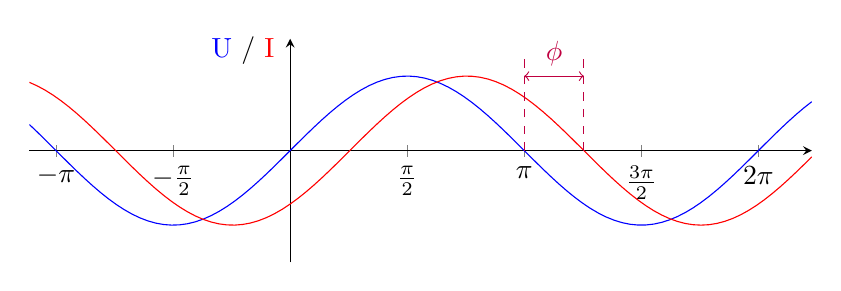
\begin{tikzpicture}
	\begin{axis}[
		axis lines=middle,
		unit vector ratio*=1 1,
		scale=1.45,
		ymin=-1.5, ymax=1.5, xmin=-3.5, xmax=7,
		domain=-3.5:7,
		samples=100,
		ylabel={\color{blue}U} / {\color{red}I},
		ylabel style={left, yshift=-1ex, xshift=-.5ex},
		ymajorticks=false,
		xtick={ -pi, -0.5*pi, 0.5*pi, pi, 1.5*pi, 2*pi},
		xticklabels={$-\pi$, $-\frac{\pi}{2}$, $\frac{\pi}{2}$, $\pi$, $\frac{3\pi}{2}$, $2\pi$},
		disabledatascaling
	]
	\addplot [mark=none, blue] {sin(deg(x))};
	\addplot [mark=none, red] {sin(deg(x-.8))};
	
	\draw[purple, dashed] (pi, 0) -- (pi, 1.3);
	\draw[purple, dashed] (pi+0.8, 0) -- (pi+0.8, 1.3);
	\draw[<->, purple]    (pi, 1) -- node[above] {$\phi$} (pi+0.8, 1);
\end{axis}
\end{tikzpicture} \end{adjustbox}
\\\strong{Obciążenie indukcyjne}: prąd wyprzedza napięcie, $\phi > 0$, $X > 0$
\end{center} \vspace{-0.3cm}

\begin{center} \begin{adjustbox}{scale=1.0} 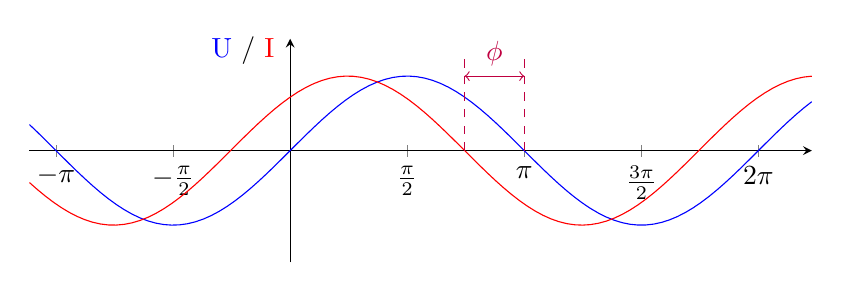
\begin{tikzpicture}
	\begin{axis}[
		axis lines=middle,
		unit vector ratio*=1 1,
		scale=1.45,
		ymin=-1.5, ymax=1.5, xmin=-3.5, xmax=7,
		domain=-3.5:7,
		samples=100,
		ylabel={\color{blue}U} / {\color{red}I},
		ylabel style={left, yshift=-1ex, xshift=-.5ex},
		ymajorticks=false,
		xtick={ -pi, -0.5*pi, 0.5*pi, pi, 1.5*pi, 2*pi},
		xticklabels={$-\pi$, $-\frac{\pi}{2}$, $\frac{\pi}{2}$, $\pi$, $\frac{3\pi}{2}$, $2\pi$},
		disabledatascaling
	]
	\addplot [mark=none, blue] {sin(deg(x))};
	\addplot [mark=none, red] {sin(deg(x+.8))};
	
	\draw[purple, dashed] (pi, 0) -- (pi, 1.3);
	\draw[purple, dashed] (pi-0.8, 0) -- (pi-0.8, 1.3);
	\draw[<->, purple]    (pi, 1) -- node[above] {$\phi$} (pi-0.8, 1);
\end{axis}
\end{tikzpicture} \end{adjustbox}
\\\strong{Obciążenie pojemnościowej}: prąd opóźniony względem napięcia, $\phi < 0$, $X < 0$
\end{center} \vspace{-0.3cm}

% https://www.falstad.com/circuit/circuitjs.html?cct=$+1+0.000005+2.803162489452614+42+1+50%0Ar+240+160+240+240+0+2.1%0Ac+544+240+544+304+0+0.00014000086000000002+0.6579358617395383%0Av+112+160+112+304+0+1+40+5+0+0+0.5%0Aw+176+304+240+304+0%0Aw+112+160+176+160+2%0Aw+240+160+176+160+1%0Aw+176+304+112+304+0%0Ag+112+304+112+336+0%0Al+240+240+240+304+0+0.012575+-0.925073781350406%0Ag+416+304+416+336+0%0Aw+480+304+416+304+0%0Aw+544+160+480+160+1%0Aw+416+160+480+160+2%0Aw+480+304+544+304+0%0Av+416+160+416+304+0+1+40+5+0+0+0.5%0Ar+544+160+544+240+0+2.1%0Ao+2+32+0+12291+5+1.5259020248913013+0+2+2+3%0Ao+14+32+0+12291+5+0.17545196169957122+0+2+14+3%0A38+8+0+0.0001+0.05+LR%5CsInductance%0A38+1+0+1e-8+0.0005+RC%5CsCapacitance%0A

\subsection{Moc pozorna, czynna i bierna}

\subsubsection{Moc pozorna}

Moc pozorna jest sumą wektorową mocy czynnej i biernej.
Związana jest ona z wartością przepływu prądu i stanowi iloraz wartości skutecznych napięcia i natężenia prądu. Wyrażana jest w wolto-amperach [VA].

\begin{center} \begin{adjustbox}{scale=0.8} \begin{tikzpicture}
	\tikzstyle{invisibleNode}=[inner sep=0, outer sep = 0pt, minimum size=0]
	\begin{axis}[
		axis lines=middle,
		xmin=-0.3, xmax=2.9,
		ymin=-0.3, ymax=2.1,
		xmajorticks=false,
		ymajorticks=false,
		xlabel={$P$ [W]},
		ylabel={$Q$ [Var]},
		xlabel style={below, xshift=-1ex},
		ylabel style={left, yshift=-1ex, xshift=-2.5ex},
		disabledatascaling
	]
		\node[invisibleNode] at (2.5,1.8) (S) {};
		
		\draw[->, line width=0.35mm, >={Stealth[length=8pt,width=6pt]}, red]   (0,0) -- node[above,yshift=2ex] {$S$ [VA]} (S);
		\draw[->, line width=0.35mm, >={Stealth[length=8pt,width=6pt]}, blue]  (0,0) -- node[below] {$P$} (S |- 0,0);
		\draw[->, line width=0.35mm, >={Stealth[length=8pt,width=6pt]}, green] (0,0) -- node[anchor = east] {$Q$} (S -| 0,0);
		
		\draw ([shift=(0:1.3)]0,0) arc (0:36:1.3);
		\node at (0.9, 0.27) {$\phi$};
		
		\draw[gray, dashed] (S) -- (S |- 0,0);
		\draw[gray, dashed] (S) -- (S -| 0,0);
		
		\node[align=center] at (1.75, -2) {\small $Z$ ma charkter\\indukcyjny};
	\end{axis}
\end{tikzpicture} \end{adjustbox} \end{center}

	$$S = \sqrt{P^2 + Q^2}$$
	$$S = U_{sk} I_{sk} = |Z| {I_{sk}}^2 = \frac{{U_{sk}}^2}{|Z|}$$

\subsubsection{Moc czynna}

Moc czynna związana jest z możliwością wykonania pracy. jest to moc tracona na części rezystancyjnej impedancji.
Wyrażana jest w watach [W].

	$$P = U_{sk} I_{sk} \cos(\phi)$$

\subsubsection{Moc bierna}

Moc bierna jest to moc przepływająca za sprawą części reaktancyjnej impedncji.
Nie jest zdolna do wykonania pracy (jest magazynowana w polu elektrycznym / magnetycznym i oddawana z powrotem do układu).
Wyrażana jest w varach [var].

	$$Q = U_{sk} I_{sk} \sin(\phi)$$

\subsubsection{Współczynnik mocy}

Mianem współczynnika mocy (\textit{PF} – power factor) określa się cosinus fi:
	$$\cos(\phi) = \frac{P}{S}$$
W energetyce często stosowany jest też tangens fi:
	$$\tan(\phi) = \frac{Q}{P}$$
